\documentclass[a0paper,portrait]{baposter}



\usepackage{wrapfig}
\usepackage{lmodern}

\usepackage[utf8]{inputenc} %unicode support
\usepackage[T1]{fontenc}

\usepackage{tikz}
\usetikzlibrary{bayesnet}
\usepackage[nopar]{lipsum}

\selectcolormodel{cmyk}

\graphicspath{{figures/}} % Directory in which figures are stored


%%%%%% math commands


\usepackage{amsmath,amsfonts,amssymb,amsthm}

\usepackage{bm}
\usepackage{hyperref}

\newcommand{\tr}{\intercal}
\newcommand{\eye}{\mathrm{I}}
\newcommand\given[1][]{\:#1\vert\:}

\newcommand{\transpose}[1]{#1^{\intercal}}
\newcommand{\R}{\mathbb{R}}
\newcommand{\nprod}{\prod\limits_{n}}
\newcommand{\kprod}{\prod\limits_{k}}
\newcommand{\nsum}{\sum\limits_{n}}
\newcommand{\ksum}{\sum\limits_{k}}
\newcommand{\boldbeta}{\boldsymbol\beta}
\newcommand{\boldgamma}{\boldsymbol\gamma}
\newcommand{\boldtau}{\boldsymbol\tau}
\newcommand{\sumexp}{\sum_{j=1}^{K} e^{ \transpose{x_n} \gamma_j}}
\newcommand{\E}{\mathbb{E}}
\newcommand{\diagdots}{_{^{\big\cdot}\cdot _{\big\cdot}}}
% \newcommand{\var}{\mathrm{Var}}

\newcommand{\betad}{\tilde{\beta}_d}
\newcommand{\betaj}{\tilde{\beta}_j}
\newcommand{\umat}{\mathrm{U}}
\newcommand{\qmat}{\mathrm{Q}}

\newcommand{\priorbeta}{\mathcal{N} \left( \betad \given 0, \xi_0^{-1} \cdot \mathrm{I}_K \right)}
\newcommand{\qbeta}{\mathcal{N} \left( \betad \given m_d, \qmat_d^{-1} \right)}


\usepackage{setspace}
\let\Algorithm\algorithm
\renewcommand\algorithm[1][]{\Algorithm[#1]\setstretch{1.05}}


\newcommand{\pr}[1]{p \left( #1 \right)}
\newcommand{\trace}[1]{\mathrm{tr} \left( #1 \right)}
\newcommand{\var}[1]{\mathrm{Var}\left(#1\right)}

%%%%%% math commands



\newcommand{\compresslist}{%
\setlength{\itemsep}{0pt}%
\setlength{\parskip}{1pt}%
\setlength{\parsep}{0pt}%
}

\newenvironment{boenumerate}
  {\begin{enumerate}\renewcommand\labelenumi{\textbf\theenumi.}}
  {\end{enumerate}}



\begin{document}


%\definecolor{darkgreen}{cmyk}{0.8,0,0.8,0.45}
\definecolor{darkgreen}{cmyk}{0.52, 0.25, 0, 0.66}
\definecolor{lightgreen}{cmyk}{0.52, 0.25, 0, 0.35}

\begin{poster}
{
grid=false,
headerborder=open, % Adds a border around the header of content boxes
colspacing=1em, % Column spacing
bgColorOne=white, % Background color for the gradient on the left side of the poster
bgColorTwo=white, % Background color for the gradient on the right side of the poster
borderColor=darkgreen, % Border color
headerColorOne=lightgreen, % Background color for the header in the content boxes (left side)
headerColorTwo=lightgreen, % Background color for the header in the content boxes (right side)
headerFontColor=white, % Text color for the header text in the content boxes
boxColorOne=white, % Background color of the content boxes
textborder=rounded, %rectangle, % Format of the border around content boxes, can be: none, bars, coils, triangles, rectangle, rounded, roundedsmall, roundedright or faded
eyecatcher=false, % Set to false for ignoring the left logo in the title and move the title left
headerheight=0.11\textheight, % Height of the header
headershape=rounded, % Specify the rounded corner in the content box headers, can be: rectangle, small-rounded, roundedright, roundedleft or rounded
headershade=plain,
headerfont=\Large\textsf, % Large, bold and sans serif font in the headers of content boxes
%textfont={\setlength{\parindent}{1.5em}}, % Uncomment for paragraph indentation
linewidth=2pt % Width of the border lines around content boxes
}
{}
%
%----------------------------------------------------------------------------------------
%	TITLE AND AUTHOR NAME
%----------------------------------------------------------------------------------------
%
{
\textsf %Sans Serif
{Variational Inference for Bayesian Density Regression.
}
} % Poster title
% {\vspace{1em} Marta Stepniewska, Pawel Siedlecki\\ % Author names
% {\small \vspace{0.7em} Department of Bioinformatics, Institute of Biochemistry and Biophysics, PAS, Warsaw, Pawinskiego 5a}} % Author email addresses
{\sf\vspace{-0.2em}\\
Eric Chuu
\vspace{0.1em}\\
\small{Department of Statistics, Texas A&M University
\vspace{0.1em}\\
ericchuu@tamu.edu}\\
\vspace{-2cm}
}
% {
\includegraphics{logo}} % University/lab logo


\headerbox{1. Introduction}{name=introduction,column=0,row=0, span=3}{
In the Bayesian density regression problem, we observe data $\left(y_n, x_n \right), n=1, \ldots, N$, and the goal is the estimate the conditional density of $y \given x$. We model the density using a mixture of Gaussians for which covariates enter the weights through a logit link function. \vspace{-3mm}
$$
	 f(y \given x) = \sum_{k}^{K} \pi_k(x) \cdot \mathcal{N} \left( y \given \mu_k(x), \tau_k^{-1} \right) \vspace{-3mm}
$$
where $\mu_k(x) = \transpose{x} \beta_k$ and $\pi_{k}(x) \propto \exp(\transpose{x} \gamma_k)$. While this increases the flexibility of the model, it also increases the computational complexity. In order to perform scalable inference on the model parameters, we propose a variational approach that uses a tangential approximation of the softmax function to achieve fast, closed form updates for the coordinate ascent algorithm. 
}

\headerbox{2. Notation}{name=notation,column=0,below = introduction, span=1}{
\begin{itemize} \setlength\itemsep{0.07em}
	\item Data: $\mathbf{y} = \{y_{1:N} \}, \mathbf{X} = \{ x_{1:N} \} \subseteq \R^{D}$
	\item Coefficients: $\boldbeta = \{ \beta_{1:K} \}, \boldgamma = \{ \gamma_{1:K} \}$ 
	\item Precision (Gaussian): $\boldtau = \{ \tau_{1:K} \}$
	\item Cluster Indicator: $\mathbf{Z} = \{ z_{1:N} \} \subseteq \R^K$
\end{itemize}
  \begin{center}
  \tikz{ %
    \node[latent] (gamma) {$\gamma$} ; %
    \node[latent, right=of gamma] (z) {$z_n$} ; %
    \node[obs, right=of z] (yn) {$y_n$} ; %
    \node[det, below =of yn] (xn) {$x_n$};
    \node[latent, right=of xn] (tau) {$\tau$} ; %
    \node[latent, right=of yn] (beta) {$\beta$} ; %
    \plate[inner sep=0.2cm, xshift=-0.12cm, yshift=0.04cm] {plate1} {(z) (yn) (xn)} {N}; %
    \edge {gamma} {z} ; %
    \edge {z,tau,beta} {yn} ; %
    \edge {beta} {yn} ; %
    \edge {tau} {beta} ; %
    \edge {xn} {yn}
    \edge {xn} {z}
  }
  \end{center}
}


\headerbox{3. Model Setup}{name=model,column=1,below=introduction,span=1}{
We use conjugate priors to ease computation.
\vspace{-2mm}
\begin{align*}
	p \left( \mathbf{y} \given \mathbf{X}, \boldsymbol\beta, \boldsymbol{\tau}, \mathbf{Z} \right) &= 
	\prod_{n} \prod_{k} \mathcal{N} \left( y_n \given \transpose{x_n} \beta_k, \tau_{k}^{-1} \right)^{z_{nk}} \\
	p \left( \mathbf{Z} \given \mathbf{X}, \boldsymbol\gamma \right) &= 
	\nprod \kprod \Bigg[ \frac{e^{\transpose{x_n} \gamma_k}}{\sumexp}\Bigg]^{z_{nk}} \\
	p \left( \boldgamma \right) &= \prod_{k} \mathcal{N} \left( \gamma_k \given 0, \eye_{D} \right) \\
	p \left( \boldbeta, \boldtau \right) &= \prod_{k} p \left(\beta_k \given \tau_k \right) p\left(\tau_k\right) \\
	p \left( \beta_k\given \tau_k \right) &= \mathcal{N} \left( \beta_k \given m_0, \left(\tau_k \Lambda_0\right)^{-1} \right) \\
	p\left(\tau_k \right) &= \mathrm{Gamma} \left( \tau_k \given a_0, b_0 \right)
\end{align*}
}


\headerbox{4. Variational Approximation}{name=variational,column=2,below=introduction,span=1}{

% \textbf{Full joint distribution:} $\pr{\mathbf{y}, \mathbf{X}, \boldbeta, \boldtau, \mathbf{Z}}$
We approximate the posterior distribution with: \vspace{-2mm}
$$q \left( \mathbf{Z}, \boldbeta, \boldtau, \boldgamma \right) = q(\mathbf{Z}) q(\boldbeta, \boldtau, \boldgamma) $$
Then the distribution for each of the variational parameters can be found by taking the expectation of the joint likelihood with respect the \textit{other} variational parameters. 
\vspace{-2mm}
\setlength{\belowdisplayskip}{5pt}%
\begin{align*}
	q^{\star}(z_{nk}) &= r_{nk}^{z_{nk}} \\
 	q^{\star}(\gamma_k) &= \mathcal{N} \left(\gamma_k \given \mu_k, \mathrm{Q}_k^{-1} \right) \\
 	q^{\star}(\beta_k \given \tau_k) &= \mathcal{N}\left(\beta_k \given m_k, (\tau_k \mathrm{V}_k)^{-1} \right) \\
 	q^{\star}(\tau_k) &=  \mathrm{Ga}\left( \tau_k \given a_k, b_k \right)
\end{align*} 
An issue arises in calculating $q(z_{nk})$ because it requires computing: \vspace{-2mm}
$$\varepsilon_n = \mathbb{E}_{q(\boldsymbol\gamma)}\Bigg[\ln \sum_{j} \exp \{ x_n^{\tr} \gamma_j \}\Bigg]$$
which is not available in closed form. We resort to the following bound (Bouchard, 2007)  \vspace{-2mm}
\setlength{\belowdisplayskip}{8pt}%
\begin{align*}
	& \varepsilon_n  \leq  \alpha_n + \sum_{j}^K \frac{1}{2}\left(x_n^{\tr}\mu_j - \alpha_n - \xi_{nj}\right) \\ & \qquad \qquad \qquad + \log( 1 + e^{\xi_{nj}})
\end{align*}
Two additional variational parameters: \vspace{-1mm}
\setlength{\belowdisplayskip}{3pt}%
\begin{align*}
    \xi_{nj} & = \sqrt{\left(\mu_j^{\intercal}x_n - \alpha_n \right)^2 + x_n^{\intercal} \mathrm{Q}_j^{-1} x_n} \\[0.9ex]
    \alpha_n & = \frac{\frac{1}{2}\left( \frac{K}{2} - 1\right) + \sum_{j = 1}^K \lambda \left( \xi_{nj} \right)\mu_j^{\intercal} x_n}{\sum_{j=1}^{K} \lambda \left( \xi_{nj}\right)} 
\end{align*}
$\vspace{-2mm} \lambda(\xi) = \frac{1}{4\xi} \tanh \left( \frac{\xi}{2} \right)$ \\

}

\headerbox{5. Application to Bimodal Conditional Densities}{name=bimodal,span=2,column=0,below=model}{ % To reduce this block to 1 column width, remove 'span=2'

For the conditional density, $X \sim \mathcal{N}(0,1), Y \given X \sim 0.5 \mathcal{N}\left( X - 1.5, 0.5^2) + 0.5 \mathcal{N} \left( X + 1.5, 1^2 \right)$, we examine samples of size 1000 and look at the conditional density at the three quartiles of the predictor support: $x = -0.6745$ (left), $x = 0$ (center), $x = 0.6475$ (right). For a sample size of 1000, we plot the approximations below. The true density is a dashed green line, the variational approximation is in red, and the kernel density estimate is in blue. 
%For each quartile, the variational algorithm does very well in finding the both modes, while the kernel density estimate is not as smooth and is more biased. Another advantage of the variational algorithm is the computational speed, which converges in seconds, while the kernel-based estimate takes more than 10 times as long.
\begin{center}
\hspace{0pt}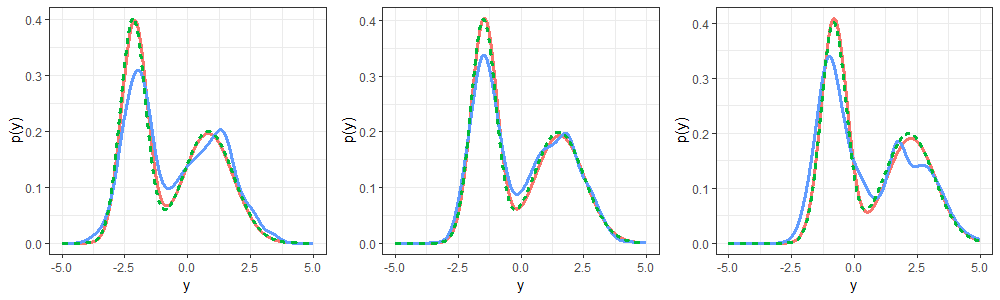
\includegraphics[width=0.95\linewidth]{unimodal_N1000}
\end{center}



% \vspace{-5pt}


}


\headerbox{6. Application to Speedflow Data}{name=sea,span=3,column=0,below=bimodal, above = bottom}{ % To reduce this block to 1 column width, remove 'span=2'

We consider the following bimodal conditional density, $X \sim \mathcal{N}(0,1), Y \given X \sim 0.5 \mathcal{N}\left( X - 1.5, 0.5^2) + 0.5 \mathcal{N} \left( X + 1.5, 0.5^2 \right)$ In particular, we look at the conditional density at the three quartiles of the predictor support: $x = -0.6745$ (left), $x = 0$ (center), $x = 0.6475$ (right). For a sample size of 1000, we plot the approximations below, where the true conditional density is a dashed green line, the variational approximation is shown in red, and the kernel density estimate is shown in blue. 
%For each quartile, the variational algorithm does very well in finding the both modes, while the kernel density estimate is not as smooth and is more biased. Another advantage of the variational algorithm is the computational speed, which converges in seconds, while the kernel-based estimate takes more than 10 times as long.
\begin{center}
\hspace{0pt}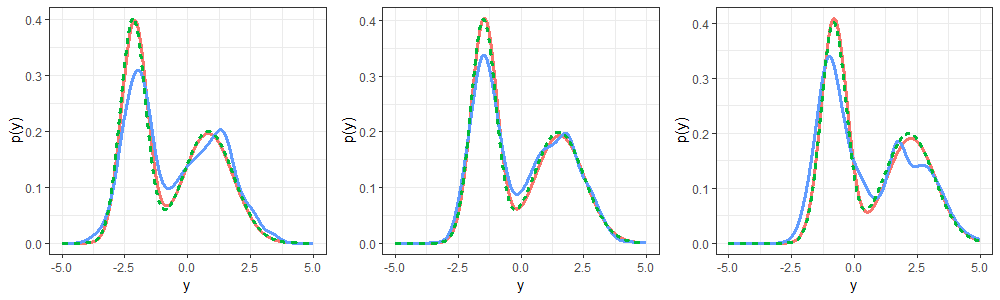
\includegraphics[width=0.75\linewidth]{unimodal_N1000}
\end{center}

}


%\headerbox{6. Extension of Algorithm via Variable Selection}{name=conclusion,column=1,below=sea,span=2,above=bottom}{
% DeCAF is a chemoinformatical tool that can be helpful in ligand-based drug design.
% It provides a comprehensive molecule description and a fast algorithms for comparing and aligning multiple ligands.
%We proved that DeCAF is a significant improvement over the SEA algorithm, a popular method for comparing sets of ligands.
%\begin{boenumerate}\compresslist
%    \item DeCAF gives better results for 23 out of 35 receptors.
%    \item For targets with easily separable active and inactive datasets, SEA and DeCAF give similar results.
%    \item In cases in which SEA fails to identify active molecules, our method performs substantially better.
%\end{boenumerate}
% It can be also used in other [procedures], such as database screening or drug repositioning.
% DeCAF is written in Python and freely available at \textbf{\color{darkgreen}http://bitbucket.org/marta-sd/decaf}. 
%}


%\headerbox{6. Variable Selection}{name=vs,column=0,span=1,below=model,above=bottom}{

%\small % Reduce the font size in this block
% \renewcommand{\section}[2]{\vskip 0.05em} % Get rid of the default "References" section title
%\nocite{*} % Insert publications even if they are not cited in the poster





\bibliographystyle{unsrt}
\bibliography{poster} % Use sample.bib as the bibliography file
}

\end{poster}

\end{document}
